% CSE 713 — Artificial Intelligence
% Topic 1: Intelligent Agents + Environments — Complete Model Answers (2020–2024)
% University of Chittagong, 7th Semester B.Sc. Engineering
%
% Compile with: pdflatex Agent_Solutions.tex (run twice for TOC)

\documentclass[12pt, a4paper]{article}

\usepackage[left=2.5cm, right=2.5cm, top=2.8cm, bottom=2.8cm, headheight=15pt]{geometry}
\usepackage{amsmath, amssymb}
\usepackage{tikz}
\usetikzlibrary{arrows.meta, positioning, shapes.geometric, calc, backgrounds, fit}
\usepackage{booktabs}
\usepackage{array}
\usepackage{xcolor}
\usepackage{enumitem}
\usepackage{fancyhdr}
\usepackage{titlesec}
\usepackage{mdframed}
\usepackage{multicol}
\usepackage{tabularx}
\usepackage{multirow}
\usepackage{hyperref}

%----- Colours -----
\definecolor{sectionblue}{RGB}{10,60,110}
\definecolor{boxbg}{RGB}{242,247,255}
\definecolor{answerbg}{RGB}{240,255,240}
\definecolor{notesbg}{RGB}{255,250,230}
\definecolor{keyblue}{RGB}{0,80,160}
\definecolor{accent}{RGB}{180,40,40}

%----- Box environments -----
\mdfdefinestyle{solutionframe}{linecolor=sectionblue, backgroundcolor=boxbg, roundcorner=4pt, linewidth=1.4pt, innertopmargin=7pt, innerbottommargin=7pt, innerleftmargin=9pt, innerrightmargin=9pt}
\mdfdefinestyle{answerframe}{linecolor=green!55!black, backgroundcolor=answerbg, roundcorner=4pt, linewidth=1.4pt, innertopmargin=7pt, innerbottommargin=7pt, innerleftmargin=9pt, innerrightmargin=9pt}
\mdfdefinestyle{notesframe}{linecolor=orange!70!black, backgroundcolor=notesbg, roundcorner=4pt, linewidth=1pt, innertopmargin=5pt, innerbottommargin=5pt, innerleftmargin=8pt, innerrightmargin=8pt}
\newenvironment{solutionbox}{\begin{mdframed}[style=solutionframe]}{\end{mdframed}}
\newenvironment{answerbox}{\begin{mdframed}[style=answerframe]}{\end{mdframed}}
\newenvironment{notesbox}{\begin{mdframed}[style=notesframe]}{\end{mdframed}}

%----- Page style -----
\pagestyle{fancy}
\fancyhf{}
\lhead{\small\color{sectionblue} CSE 713 — Topic 1: Intelligent Agents \& Environments}
\rhead{\small\color{sectionblue} Model Solutions (2020–2024)}
\cfoot{\small\thepage}
\renewcommand{\headrulewidth}{0.5pt}

%----- Section formatting -----
\titleformat{\section}{\Large\bfseries\color{sectionblue}}{}{0em}{}[\vspace{-2pt}\color{sectionblue}\rule{\linewidth}{0.8pt}]
\titleformat{\subsection}{\large\bfseries\color{sectionblue!85!black}}{}{0em}{}
\titleformat{\subsubsection}{\normalsize\bfseries\color{black}}{}{0em}{}

%----- Custom list -----
\newlist{keypoints}{itemize}{1}
\setlist[keypoints]{label=$\triangleright$, leftmargin=1.5cm, itemsep=2pt, topsep=3pt}
\newlist{examlist}{enumerate}{1}
\setlist[examlist]{label=\textbf{(\roman*)}, leftmargin=1.8cm, itemsep=3pt, topsep=4pt}

%----- Macros -----
\newcommand{\qpart}[1]{\textbf{#1}}
\newcommand{\hdr}[1]{\vspace{0.4em}\noindent\textbf{\color{keyblue}#1}\vspace{0.2em}}

%=====================================================================
\begin{document}
%=====================================================================

\begin{center}
  {\LARGE\bfseries\color{sectionblue} CSE 713: Artificial Intelligence}\\[0.6em]
  {\Large\bfseries Topic 1 — Intelligent Agents \& Environments}\\[0.3em]
  {\large Complete Model Answers (2020–2024)}\\[0.2em]
  {\normalsize University of Chittagong \quad|\quad 7\textsuperscript{th} Semester B.Sc.\ (Engg.) Examination}\\[0.3em]
  {\small Source: Ch01-02.pdf (Russell \& Norvig, Chapters 1--2)}
\end{center}

\vspace{0.3em}
\noindent\rule{\linewidth}{1pt}
\vspace{0.5em}

\tableofcontents
\newpage

%=====================================================================
\section{Theoretical Framework — Reusable Across All Years}
%=====================================================================

This section covers the \textbf{core theory} that appears in every year's Q1. Master these concepts once — they are the building blocks for answering ANY agent–environment question.

%----------------------------------------------------------------------
\subsection{What is Artificial Intelligence?}
%----------------------------------------------------------------------

\noindent AI can be defined along \textbf{two dimensions} (thought/reasoning vs.\ behaviour) and \textbf{two goals} (human-like vs.\ rational/ideal):

\begin{center}
\renewcommand{\arraystretch}{1.6}
\begin{tabular}{p{5.5cm}|p{5.5cm}|p{5.5cm}}
\toprule
& \textbf{Human-Centred} & \textbf{Rationality-Centred} \\
\midrule
\textbf{Thought / Reasoning} &
  \textbf{Thinking Humanly} \\
  Cognitive modelling — replicate human thought processes. \\
  \emph{Example:} ACT-R, SOAR cognitive architectures. &
  \textbf{Thinking Rationally} \\
  Formal logic — follow laws of thought. \\
  \emph{Example:} Syllogisms, first-order logic, theorem provers. \\
\midrule
\textbf{Behaviour / Action} &
  \textbf{Acting Humanly} \\
  Turing Test approach — behave indistinguishably from humans. \\
  \emph{Example:} Chatbots, NLP systems. &
  \textbf{Acting Rationally} \\
  Rational agent approach — act to achieve best outcome given beliefs. \\
  \emph{Example:} Self-driving cars, game-playing AI, Mars rovers. \\
\bottomrule
\end{tabular}
\end{center}

\begin{answerbox}
\textbf{Exam definition (memorise):} AI is the study and design of \textbf{rational agents} — systems that perceive their environment through sensors and act upon it through actuators to maximise their performance measure, given the available knowledge and computational resources.
\end{answerbox}

\subsubsection*{AI vs Machine Learning vs Deep Learning}

\begin{center}
\renewcommand{\arraystretch}{1.3}
\begin{tabular}{l|p{10cm}}
\toprule
\textbf{AI} & The broad field — building systems that exhibit intelligent behaviour. Encompasses search, reasoning, planning, learning, perception, NLP, robotics. \\
\textbf{Machine Learning} & A subset of AI — systems that learn patterns from data without being explicitly programmed for every rule. \\
\textbf{Deep Learning} & A subset of ML — uses multi-layer neural networks to learn hierarchical representations from large datasets. \\
\bottomrule
\end{tabular}
\end{center}

\noindent \textbf{One-liner:} AI is the goal (intelligent machines); ML is the method (learning from data); DL is the tool (deep neural nets).

%----------------------------------------------------------------------
\subsection{The Turing Test}
%----------------------------------------------------------------------

\noindent Proposed by Alan Turing (1950) in \textit{Computing Machinery and Intelligence}.

\vspace{0.3em}
\noindent\textbf{Setup:} A human interrogator communicates (via text) with two entities — one human, one machine. If the interrogator cannot reliably distinguish the machine from the human after a conversation, the machine is said to exhibit \textbf{human-level intelligence}.

\vspace{0.4em}
\noindent\textbf{Capabilities a machine must have to pass the Turing Test:}
\begin{keypoints}
  \item \textbf{Natural Language Processing (NLP):} Understand and generate human language.
  \item \textbf{Knowledge Representation:} Store and retrieve what it knows.
  \item \textbf{Automated Reasoning:} Draw inferences from stored knowledge to answer novel questions.
  \item \textbf{Machine Learning:} Adapt to new circumstances, detect patterns, learn from interaction.
  \item \textbf{(Optional) Computer Vision + Robotics:} For the \emph{Total} Turing Test, the machine must also perceive and manipulate physical objects.
\end{keypoints}

\vspace{0.4em}
\noindent\textbf{Why modern LLMs (ChatGPT, GPT-4, Claude) still fail the Turing Test in extended interactions:}
\begin{keypoints}
  \item \textbf{No real-world grounding:} LLMs process tokens, not physical experiences. They have never seen a sunset, felt pain, or interacted with objects.
  \item \textbf{Hallucinations:} Confidently generate false information with no awareness of doing so.
  \item \textbf{No stable long-term memory:} Each conversation is stateless (unless explicitly managed). No persistent identity or autobiographical continuity.
  \item \textbf{Long-horizon dialogue failure:} Over many turns, LLMs lose coherence, contradict earlier statements, and fail to maintain consistent goals.
  \item \textbf{No genuine intentionality:} LLMs predict tokens — they don't \emph{believe}, \emph{desire}, or \emph{intend} in any philosophical sense.
\end{keypoints}

%----------------------------------------------------------------------
\subsection{Intelligent Agents — Core Concepts}
%----------------------------------------------------------------------

\subsubsection*{Agent Definition}

\noindent An \textbf{agent} is anything that \textbf{perceives} its environment through \textbf{sensors} and \textbf{acts} upon it through \textbf{actuators}. The \textbf{agent function} $f : P^* \to A$ maps every possible percept sequence to an action.

\vspace{0.3em}
\noindent\textbf{Rational Agent:} For each possible percept sequence, a rational agent selects an action expected to \textbf{maximise its performance measure}, given:
\begin{enumerate}[noitemsep]
  \item The percept sequence it has observed so far.
  \item Its built-in prior knowledge about the environment.
  \item The actions it can perform.
\end{enumerate}

\subsubsection*{PAGE Model}

\noindent Every agent scenario can be analysed using the \textbf{PAGE} framework:

\begin{center}
\renewcommand{\arraystretch}{1.3}
\begin{tabular}{l|p{12cm}}
\toprule
\textbf{P} & \textbf{Percepts} — Sensory inputs. What does the agent perceive? \emph{(cameras, microphones, LIDAR, temperature, GPS, touch, etc.)} \\
\textbf{A} & \textbf{Actions} — Outputs/actuators. What can the agent do? \emph{(move, speak, display, grab, send signal, etc.)} \\
\textbf{G} & \textbf{Goals} — Desired states of the world the agent aims to achieve. \emph{(clean room, reach destination, maximise crop yield, etc.)} \\
\textbf{E} & \textbf{Environments} — The world in which the agent operates, characterised by 6 dimensions. \\
\bottomrule
\end{tabular}
\end{center}

%----------------------------------------------------------------------
\subsection{Five Agent Architectures (Ordered by Sophistication)}
%----------------------------------------------------------------------

\begin{enumerate}[leftmargin=1.2cm, itemsep=6pt]

  \item \textbf{Simple Reflex Agent}
  \begin{itemize}[noitemsep]
    \item Selects actions based on the \textbf{current percept only}, ignoring percept history.
    \item Uses \textbf{condition–action rules}: IF \textit{condition} THEN \textit{action}.
    \item \textbf{Limitation:} Cannot handle partial observability — needs full state in current percept.
    \item \textbf{Works in:} Fully observable environments (e.g., thermostat, spam filter).
  \end{itemize}

  \item \textbf{Model-Based Reflex Agent}
  \begin{itemize}[noitemsep]
    \item Maintains an \textbf{internal state} that tracks how the world evolves and how its own actions affect the world — a \textbf{world model}.
    \item Handles \textbf{partial observability} by filling in missing information from the model.
    \item \textbf{Works in:} Partially observable environments (e.g., a robot that remembers object positions after they leave its camera view).
  \end{itemize}

  \item \textbf{Goal-Based Agent}
  \begin{itemize}[noitemsep]
    \item In addition to the world model, maintains \textbf{explicit goals} — descriptions of desired situations.
    \item Considers \textbf{future consequences} of actions: ``Will this get me closer to my goal?''
    \item Requires \textbf{search or planning} to find action sequences that achieve the goal.
    \item \textbf{Works in:} Environments where the right action depends on long-term consequences (e.g., navigation, puzzle-solving).
  \end{itemize}

  \item \textbf{Utility-Based Agent}
  \begin{itemize}[noitemsep]
    \item Extends goal-based agents with a \textbf{utility function} — maps states to real numbers measuring ``happiness'' or ``preference.''
    \item Can handle \textbf{trade-offs} between conflicting goals and \textbf{uncertainty} about outcomes.
    \item Selects the action that \textbf{maximises expected utility}.
    \item \textbf{Works in:} Stochastic environments with multiple, possibly conflicting, objectives (e.g., autonomous taxi: safety vs.\ speed vs.\ comfort vs.\ fuel economy).
  \end{itemize}

  \item \textbf{Learning Agent}
  \begin{itemize}[noitemsep]
    \item Can become more competent over time through experience.
    \item \textbf{Four components:}
    \begin{enumerate}[noitemsep]
      \item \textbf{Performance element} — selects external actions (the ``acting'' part).
      \item \textbf{Critic} — evaluates how well the agent is doing against a fixed performance standard; provides feedback to the learning element.
      \item \textbf{Learning element} — uses feedback from the critic to improve the performance element.
      \item \textbf{Problem generator} — suggests exploratory actions that may be suboptimal short-term but lead to better long-term performance.
    \end{enumerate}
    \item \textbf{Works in:} Unknown or changing environments where the agent must adapt (e.g., recommendation systems, adaptive robots).
  \end{itemize}

\end{enumerate}

\subsubsection*{Quick Decision Table — Which Architecture?}

\begin{center}
\renewcommand{\arraystretch}{1.3}
\begin{tabular}{l|l}
\toprule
\textbf{Scenario characteristic} & \textbf{Best architecture} \\
\midrule
Fully observable, simple mapping from percept to action & Simple Reflex \\
Partially observable, need to track unseen aspects & Model-Based \\
Actions need long-term planning toward a goal & Goal-Based \\
Conflicting objectives, uncertainty, need trade-offs & Utility-Based \\
Environment unknown or changing, need adaptation & Learning \\
\bottomrule
\end{tabular}
\end{center}

%----------------------------------------------------------------------
\subsection{Six Environment Dimensions (PEAS Analysis)}
%----------------------------------------------------------------------

\begin{center}
\renewcommand{\arraystretch}{1.5}
\begin{tabular}{l|p{5cm}|p{5cm}|p{5cm}}
\toprule
\textbf{Dimension} & \textbf{Property A} & \textbf{Property B} & \textbf{Memory Aid} \\
\midrule
\textbf{1. Observability} &
  \textbf{Fully observable} \\
  Agent's sensors give complete state at all times. &
  \textbf{Partially observable} \\
  Sensors are noisy, limited, or miss relevant data. &
  \emph{Can the agent see everything?} \\
\midrule
\textbf{2. Determinism} &
  \textbf{Deterministic} \\
  Next state completely determined by current state + action. &
  \textbf{Stochastic} \\
  Next state has a random element. \\
  \textbf{Strategic} (special case): deterministic except for actions of other agents. &
  \emph{Is the next state predictable?} \\
\midrule
\textbf{3. Episodicity} &
  \textbf{Episodic} \\
  Each action–percept episode is independent. No effect on future episodes. &
  \textbf{Sequential} \\
  Current actions affect all future decisions. Requires long-term planning. &
  \emph{Do my actions now affect my future?} \\
\midrule
\textbf{4. Dynamism} &
  \textbf{Static} \\
  Environment does not change while agent is deliberating. &
  \textbf{Dynamic} \\
  Environment can change during deliberation. Agent must keep up. \\
  \textbf{Semi-dynamic}: Environment static but performance score changes with time. &
  \emph{Does the world wait for me?} \\
\midrule
\textbf{5. Continuity} &
  \textbf{Discrete} \\
  Finite, distinct set of percepts and actions. &
  \textbf{Continuous} \\
  Percepts and actions flow in a continuum (real numbers, time). &
  \emph{Are percepts/actions countable?} \\
\midrule
\textbf{6. Agency} &
  \textbf{Single-agent} \\
  Only one agent in the environment. &
  \textbf{Multi-agent} \\
  Multiple agents; may be \textbf{cooperative} or \textbf{competitive}. &
  \emph{Are there other agents?} \\
\bottomrule
\end{tabular}
\end{center}

\newpage

%=====================================================================
\section{Examination 2024 — Q1 (9 Marks)}
%=====================================================================

\begin{solutionbox}
\textbf{Question breakdown:}
\begin{enumerate}[noitemsep]
  \item[(a)] Define AI. Point out a few recent advancements of AI. (1)
  \item[(b)] Differentiate between AI and Machine Learning. (1.5)
  \item[(c)] Evaluate LLM performance against the Turing Test — correspondence + limitations. (2.5)
  \item[(d)] Autonomous Agricultural Field Robot — percepts, environment, actions, performance, architecture. (4)
\end{enumerate}
\end{solutionbox}

%----------------------------------------------------------------------
\subsection{Part (a) — AI Definition + Recent Advancements \ [1 mark]}
%----------------------------------------------------------------------

\subsubsection*{Definition}

\noindent Artificial Intelligence is the branch of computer science concerned with creating systems that exhibit intelligent behaviour — perceiving, reasoning, learning, and acting — to achieve goals in complex environments.

\subsubsection*{Recent Advancements (2023–2024)}

\begin{keypoints}
  \item \textbf{Large Language Models (LLMs):} GPT-4, Claude, Gemini — human-level text generation, reasoning, coding, and multi-modal understanding.
  \item \textbf{Generative AI:} DALL-E, Midjourney, Sora — text-to-image and text-to-video generation at unprecedented quality.
  \item \textbf{AI in Healthcare:} AlphaFold 3 predicting protein structures; AI-assisted diagnosis matching or exceeding radiologist accuracy.
  \item \textbf{Autonomous Systems:} Level 4 self-driving expanding to more cities (Waymo, Cruise); agricultural robots and delivery drones deployed at scale.
  \item \textbf{Multimodal AI:} Systems integrating text, vision, audio, and sensor data — enabling richer real-world understanding.
  \item \textbf{AI for Science:} AI-driven drug discovery, climate modelling, and theorem proving.
\end{keypoints}

%----------------------------------------------------------------------
\subsection{Part (b) — AI vs Machine Learning \ [1.5 marks]}
%----------------------------------------------------------------------

\begin{center}
\renewcommand{\arraystretch}{1.4}
\begin{tabular}{p{3cm}|p{6.5cm}|p{6.5cm}}
\toprule
\textbf{Aspect} & \textbf{Artificial Intelligence (AI)} & \textbf{Machine Learning (ML)} \\
\midrule
\textbf{Scope} &
  Broad field — any technique that produces intelligent behaviour. &
  Specific approach within AI — learning from data without explicit programming. \\
\midrule
\textbf{Method} &
  Includes search, logic, planning, knowledge representation, \emph{and} learning. &
  Statistical pattern recognition from examples. \\
\midrule
\textbf{Relationship} &
  AI is the superset — ML is a subset of AI. &
  ML is a method for achieving AI. \\
\midrule
\textbf{Examples} &
  Expert systems, A* pathfinding, STRIPS planning, Alpha-Beta pruning, \emph{and} neural networks. &
  Linear regression, SVMs, random forests, neural networks, reinforcement learning. \\
\midrule
\textbf{When to use} &
  When rules, logic, or search can solve the problem directly. &
  When the problem is too complex to hand-code rules — let the system learn from data. \\
\bottomrule
\end{tabular}
\end{center}

\noindent \textbf{Key insight:} Not all AI is ML. A chess engine using minimax with alpha-beta pruning is AI but not ML. A system that learns chess by playing millions of games against itself (AlphaZero) uses ML to achieve AI.

%----------------------------------------------------------------------
\subsection{Part (c) — LLMs and the Turing Test \ [2.5 marks]}
%----------------------------------------------------------------------

\subsubsection*{(i) How LLMs Correspond with Turing Test Goals}

\begin{keypoints}
  \item \textbf{Fluency:} LLMs produce grammatically perfect, coherent, contextually appropriate text across diverse topics — indistinguishable from human writing in short exchanges.
  \item \textbf{Contextual awareness:} Within a single conversation, LLMs track topic shifts, maintain pronoun references, and respond relevantly — appearing to ``understand'' the dialogue flow.
  \item \textbf{Reasoning:} Modern LLMs can solve logic puzzles, write code, analyse arguments, and answer multi-step reasoning questions — mimicking the intellectual capabilities the Turing Test was designed to probe.
  \item \textbf{Breadth of knowledge:} LLMs are trained on vast corpora and can discuss topics from quantum physics to poetry — matching or exceeding any individual human's range.
  \item \textbf{Conversational naturalness:} LLMs use humour, acknowledge uncertainty (sometimes), and adapt tone — all hallmarks of human-like conversation the Turing Test values.
\end{keypoints}

\subsubsection*{(ii) Limitations Preventing Reliable Turing Test Passage}

\begin{keypoints}
  \item \textbf{Insufficient real-world grounding:} LLMs know only tokens — they have never touched, seen, tasted, or experienced the physical world. A human can describe the feeling of sand between toes from experience; an LLM can only regurgitate descriptions it has read.
  \item \textbf{Hallucinations:} LLMs confidently fabricate facts, citations, and events. A determined interrogator asking verifiable factual questions (``What did you have for breakfast?'', ``What's the colour of the shirt you're wearing?'') would quickly expose the lack of embodied experience.
  \item \textbf{No stable memory or identity:} LLMs lack autobiographical continuity. They don't remember conversations from yesterday, have no consistent personality across sessions, and cannot reflect on a ``life'' they've lived — a key aspect of human identity.
  \item \textbf{Long-horizon dialogue failure:} Over many turns, LLMs lose coherence, contradict earlier positions, and fail to pursue consistent goals. Extended conversations reveal the statistical pattern-matching underneath.
  \item \textbf{No genuine understanding:} The Chinese Room Argument (Searle, 1980) applies strongly — LLMs manipulate symbols according to statistical rules without any genuine comprehension, intentionality, or consciousness.
\end{keypoints}

%----------------------------------------------------------------------
\subsection{Part (d) — Autonomous Agricultural Field Robot \ [4 marks]}
%----------------------------------------------------------------------

\begin{solutionbox}
\textbf{Scenario:} A robot deployed in Bangladeshi farmlands to monitor crop health, detect pest infestations, and spray fertiliser/pesticide autonomously.
\end{solutionbox}

\subsubsection*{(i) Sensory Inputs (Percepts)}

\begin{keypoints}
  \item \textbf{Visual:} RGB and multi-spectral cameras for crop health assessment (NDVI), pest detection, and weed identification.
  \item \textbf{Environmental:} Temperature, humidity, soil moisture sensors.
  \item \textbf{Positional:} GPS for field navigation; IMU (Inertial Measurement Unit) for orientation and balance.
  \item \textbf{Proximity:} Ultrasonic/LIDAR sensors for obstacle detection (trees, irrigation equipment, field boundaries).
  \item \textbf{Chemical:} Soil pH and nutrient sensors; fertiliser/pesticide tank level sensors.
  \item \textbf{Weather:} Barometric pressure, wind speed (relevant for spray drift).
\end{keypoints}

\subsubsection*{(ii) Environment Characterisation}

\begin{center}
\renewcommand{\arraystretch}{1.3}
\begin{tabular}{l|l|l}
\toprule
\textbf{Dimension} & \textbf{Classification} & \textbf{Justification} \\
\midrule
Observability & \textbf{Partially observable} & Sensors cannot see below soil surface, behind dense crops, or predict weather perfectly. \\
Determinism & \textbf{Stochastic} & Weather, pest behaviour, crop growth, and sensor noise introduce randomness. \\
Episodicity & \textbf{Sequential} & Each action (spraying, moving) affects future states — fertiliser applied now changes tomorrow's crop conditions. \\
Dynamism & \textbf{Dynamic} & Crops grow, pests move, weather changes — all while the robot operates. Environment does not wait. \\
Continuity & \textbf{Continuous} & Position, speed, chemical quantities, and time are all continuous variables. \\
Agency & \textbf{Single-agent} (mostly) & The robot operates independently. Other farm machinery or human workers may occasionally interact. \\
\bottomrule
\end{tabular}
\end{center}

\subsubsection*{(iii) Actions Available}

\begin{keypoints}
  \item \textbf{Navigate:} Move through crop rows following GPS waypoints; avoid obstacles.
  \item \textbf{Monitor:} Capture and analyse crop images; record sensor data at waypoints.
  \item \textbf{Spray:} Apply precise amounts of fertiliser or pesticide to targeted areas.
  \item \textbf{Report:} Transmit crop health data, pest alerts, and task completion status to a central farm management system.
  \item \textbf{Return to base:} Navigate back to charging/refilling station when battery or chemical tanks are low.
  \item \textbf{Emergency stop:} Halt all operations if a safety hazard is detected.
\end{keypoints}

\subsubsection*{(iv) Performance Evaluation}

\begin{keypoints}
  \item \textbf{Crop yield improvement:} Compare harvest output of robot-managed fields vs.\ traditionally managed control fields.
  \item \textbf{Pest detection accuracy:} Precision and recall of pest identification against human expert ground truth.
  \item \textbf{Resource efficiency:} Reduction in fertiliser/pesticide/water usage compared to blanket application methods.
  \item \textbf{Coverage completeness:} Percentage of field area adequately monitored and treated.
  \item \textbf{Operational uptime:} Hours of autonomous operation between interventions.
  \item \textbf{False positive rate:} Healthy plants incorrectly flagged as diseased.
  \item \textbf{Safety incidents:} Number of collisions, chemical spills, or crop damage events.
\end{keypoints}

\subsubsection*{(v) Most Appropriate Agent Architecture}

\begin{answerbox}
\textbf{Recommended: Learning Agent}

\noindent\textbf{Justification:}
\begin{keypoints}
  \item The agricultural environment is \textbf{complex and changing} — crop varieties, pest patterns, weather, and soil conditions vary across seasons and fields. A fixed rule-based system would quickly become obsolete.
  \item The robot must \textbf{improve over time} — learning which visual patterns truly indicate disease, which spray patterns are most effective, and which navigation routes are most efficient.
  \item A \textbf{pure model-based agent} would require an impossibly detailed model of crop biology, pest dynamics, and weather patterns. A \textbf{learning agent} can build and refine its model from data.
  \item The \textbf{critic} component evaluates outcomes (crop health weeks after spraying) and the \textbf{learning element} adjusts strategies accordingly.
  \item The \textbf{problem generator} suggests exploratory actions (testing a new spray pattern on a small sub-field) to discover better strategies.
\end{keypoints}

\noindent The learning agent architecture subsumes the capabilities of simpler architectures: it uses condition–action rules (Simple Reflex), maintains a world model (Model-Based), pursues goals like full field coverage (Goal-Based), and optimises multiple objectives — yield, efficiency, safety (Utility-Based).
\end{answerbox}

\newpage

%=====================================================================
\section{Examination 2023 — Q1 (9 Marks)}
%=====================================================================

\begin{solutionbox}
\textbf{Question breakdown:}
\begin{enumerate}[noitemsep]
  \item[(a)] Define AI. Clarify connections among AI forms through generative traits, capabilities, and functional attributes. (2)
  \item[(b)] Evaluate ChatGPT against the Turing Test — correspondence + limitations in complex interactions. (3)
  \item[(c)] Investigate Mars Rovers Curiosity (2012) and Perseverance (2021) — percepts, environment, actions, performance, architecture. (4)
\end{enumerate}
\end{solutionbox}

%----------------------------------------------------------------------
\subsection{Part (a) — AI Definition + Connections Among AI Forms \ [2 marks]}
%----------------------------------------------------------------------

\subsubsection*{Definition}

\noindent AI is the science and engineering of creating intelligent machines — especially intelligent computer programs — that can perceive, reason, learn, and act to achieve goals.

\subsubsection*{Clarifying Connections Among AI Forms}

\noindent Different forms of AI can be understood through three organising lenses:

\vspace{0.3em}
\noindent\textbf{1. Generative Traits (What is it born with?)}

\begin{center}
\renewcommand{\arraystretch}{1.2}
\begin{tabular}{l|p{12cm}}
\toprule
\textbf{Trait} & \textbf{Meaning} \\
\midrule
Reactive & Responds to current percepts only (Simple Reflex). \\
Deliberative & Reasons about future before acting (Goal-Based, Planning). \\
Learning & Improves performance from experience (Learning Agent). \\
Adaptive & Adjusts to changing environments (Model-Based + Learning). \\
Autonomous & Operates without human intervention. \\
\bottomrule
\end{tabular}
\end{center}

\vspace{0.3em}
\noindent\textbf{2. Capabilities (What can it do?)}
\begin{keypoints}
  \item \textbf{Perception:} Computer vision, speech recognition, sensor fusion — converting raw sensory data into usable representations.
  \item \textbf{Reasoning:} Logical inference, probabilistic reasoning, constraint satisfaction — drawing conclusions from knowledge.
  \item \textbf{Knowledge representation:} Ontologies, semantic networks, Bayesian networks — structuring what the system knows.
  \item \textbf{Planning:} Search, STRIPS, hierarchical planning — finding sequences of actions to achieve goals.
  \item \textbf{Learning:} Supervised, unsupervised, reinforcement — improving from data and experience.
  \item \textbf{Communication:} NLP, dialogue systems, machine translation — interacting with humans in natural language.
\end{keypoints}

\vspace{0.3em}
\noindent\textbf{3. Functional Attributes (How does it operate?)}
\begin{keypoints}
  \item \textbf{Autonomy:} Degree of independence from human control.
  \item \textbf{Generality:} Narrow AI (single task, e.g., chess) vs.\ General AI (any intellectual task a human can do).
  \item \textbf{Transparency:} White-box (explainable) vs.\ black-box (opaque neural networks).
  \item \textbf{Embodiment:} Software-only (LLM) vs.\ physically embodied (robot, self-driving car).
  \item \textbf{Interaction mode:} Offline (batch processing) vs.\ online (real-time, continuous).
\end{keypoints}

\noindent\textbf{Key insight:} These three lenses reveal that ``AI'' is not monolithic. A chess engine (narrow, deliberative, software) and a Mars rover (narrow, reactive+deliberative, embodied, learning) are both AI — but with different generative traits, capabilities, and functional attributes.

%----------------------------------------------------------------------
\subsection{Part (b) — ChatGPT and the Turing Test \ [3 marks]}
%----------------------------------------------------------------------

\subsubsection*{(i) Ways ChatGPT Corresponds to Turing Test Goals}

\begin{keypoints}
  \item \textbf{Human-like conversational emulation:} ChatGPT produces natural, coherent, context-aware dialogue indistinguishable from human text in short interactions — exactly the surface behaviour the Turing Test measures.
  \item \textbf{Knowledge retrieval and synthesis:} Answers factual questions, summarises documents, translates languages — demonstrating breadth of knowledge across domains.
  \item \textbf{Reasoning capability:} Solves puzzles, debugs code, analyses arguments — mimicking intellectual discourse.
  \item \textbf{Creative generation:} Writes poetry, stories, and essays with stylistic variation — a capability Turing specifically cited as evidence of intelligence.
  \item \textbf{Persona adaptation:} Can adopt different tones and personas — further simulating human conversational variety.
\end{keypoints}

\subsubsection*{(ii) Limitations Preventing ChatGPT from Passing Prolonged/Complex Turing Tests}

\begin{keypoints}
  \item \textbf{Context window limitations:} ChatGPT has a finite context — beyond it, earlier conversation is forgotten, leading to inconsistency that a human interrogator would detect.
  \item \textbf{Lack of genuine understanding:} ChatGPT predicts likely next tokens — it does not \emph{understand} concepts in any meaningful sense. Extended probing on a single topic often reveals shallow comprehension.
  \item \textbf{Inability to refuse impossible tasks gracefully:} Humans recognise absurd requests; ChatGPT often attempts to oblige, revealing its lack of genuine situational awareness.
  \item \textbf{No personal experience to draw from:} Questions like ``Tell me about a time you were embarrassed'' have no genuine answer — only fabricated narratives.
  \item \textbf{Emotional shallowness:} While ChatGPT can describe emotions, it cannot feel them, and sustained emotional conversation reveals hollow affect.
  \item \textbf{Factual inconsistency over time:} In multi-session interactions, ChatGPT cannot maintain consistent personal history, opinions, or relationships — a dead giveaway.
\end{keypoints}

%----------------------------------------------------------------------
\subsection{Part (c) — Mars Rovers \ [4 marks]}
%----------------------------------------------------------------------

\subsubsection*{(i) Sensory Inputs (Percepts)}

\begin{multicols}{2}
\textbf{Curiosity (2012):}
\begin{keypoints}
  \item MastCam (colour imaging)
  \item ChemCam (laser-induced spectroscopy)
  \item MAHLI (microscopic imager)
  \item REMS (weather station: temp, pressure, humidity, UV)
  \item RAD (radiation detector)
  \item DAN (neutron detector for subsurface hydrogen/water)
  \item MARDI (descent imager)
  \item Wheel odometry + IMU
\end{keypoints}

\columnbreak

\textbf{Perseverance (2021):}
\begin{keypoints}
  \item All Curiosity-class instruments, plus:
  \item SuperCam (enhanced spectroscopy + microphone)
  \item PIXL (X-ray fluorescence for elemental composition)
  \item SHERLOC (UV Raman spectrometer for organics)
  \item MOXIE (oxygen production experiment)
  \item MEDA (enhanced weather sensors + dust analysis)
  \item Ingenuity helicopter telemetry (scout imagery)
  \item 23 cameras (vs Curiosity's 17)
\end{keypoints}
\end{multicols}

\subsubsection*{(ii) Environment Characterisation}

\begin{center}
\renewcommand{\arraystretch}{1.3}
\begin{tabular}{l|l|l}
\toprule
\textbf{Dimension} & \textbf{Classification} & \textbf{Justification} \\
\midrule
Observability & \textbf{Partially observable} & Cannot see inside rocks, below surface, or behind terrain features. Dust storms obscure vision. \\
Determinism & \textbf{Stochastic} & Terrain slippage, dust accumulation on solar panels, wind gusts, communication dropouts — all unpredictable. \\
Episodicity & \textbf{Sequential} & Today's traverse affects tomorrow's position; sample collection decisions are irreversible; battery and resource management are cumulative. \\
Dynamism & \textbf{Semi-dynamic} & Martian environment changes slowly (dust storms, seasonal cycles) but not while the rover deliberates (deliberation is fast relative to environmental change). However, communication windows are time-critical. \\
Continuity & \textbf{Continuous} & Position, speed, temperature, radiation — all real-valued, continuous quantities. \\
Agency & \textbf{Single-agent} (primarily) & One rover per landing site (Curiosity at Gale Crater; Perseverance at Jezero). Ingenuity helicopter (for Perseverance) introduces limited multi-agent interaction. \\
\bottomrule
\end{tabular}
\end{center}

\subsubsection*{(iii) Actions Available}

\begin{keypoints}
  \item \textbf{Traverse:} Navigate autonomously to target waypoints using hazard-avoidance cameras and terrain analysis.
  \item \textbf{Observe:} Capture images and spectra of rocks, soil, and atmosphere.
  \item \textbf{Analyse:} Drill into rocks, collect powdered samples, perform onboard chemical/mineral analysis.
  \item \textbf{Sample (Perseverance):} Collect and cache rock/soil cores in sealed tubes for future retrieval (Mars Sample Return mission).
  \item \textbf{Communicate:} Transmit science data and telemetry to Earth via orbiters (MRO, Odyssey, MAVEN).
  \item \textbf{Survive:} Enter low-power ``sleep'' mode during dust storms or communication blackouts; manage thermal and power states.
  \item \textbf{Self-diagnose:} Detect anomalies (wheel slip, actuator failure), report faults, enter safe mode.
\end{keypoints}

\subsubsection*{(iv) Performance Evaluation}

\begin{keypoints}
  \item \textbf{Science return:} Number and quality of analysed rock/soil samples; novel discoveries (organic molecules, ancient water evidence, biosignatures).
  \item \textbf{Distance traversed:} Total kilometres driven over mission lifetime (Curiosity: 30+ km; Perseverance: 25+ km and ongoing).
  \item \textbf{Mission duration:} Operating lifetime vs.\ planned primary mission (Curiosity: planned 2 years, operating 12+ years).
  \item \textbf{Sample cache quality (Perseverance):} Number and diversity of sealed samples ready for Earth return.
  \item \textbf{Autonomy effectiveness:} Percentage of traverse decisions made autonomously vs.\ requiring Earth-in-the-loop.
  \item \textbf{Survival:} Number of fault conditions successfully recovered from without mission loss.
  \item \textbf{Communication throughput:} Gigabits of science data successfully relayed to Earth.
\end{keypoints}

\subsubsection*{(v) Most Appropriate Agent Architecture}

\begin{answerbox}
\textbf{Recommended: Hybrid — Model-Based + Goal-Based + Learning Agent}

\noindent\textbf{Justification:}
\begin{keypoints}
  \item \textbf{Model-Based (essential):} The rover must maintain an internal model of its position, terrain map, instrument states, and power/thermal budgets because direct observation is incomplete (partially observable).
  \item \textbf{Goal-Based (essential):} Daily science goals (``drive to this rock outcrop, analyse with ChemCam, then traverse to the next waypoint'') require planning — the rover must reason about sequences of actions to achieve objectives. Simple reflex rules cannot handle the complexity of multi-kilometre autonomous navigation.
  \item \textbf{Learning (increasingly important):} Modern rovers use machine learning for: autonomous terrain classification (which surfaces are safe to drive on?), mineral identification from spectra, and adaptive path planning (learning from past wheel slip events). Perseverance's AutoNav system incorporates learned terrain preferences.
  \item \textbf{Utility function:} The rover balances competing objectives — science return vs.\ survival vs.\ communication opportunities vs.\ energy conservation — requiring utility-based decision making.
\end{keypoints}

\noindent A pure Utility-Based agent is the most comprehensive single classification, but in practice, the rover is a hybrid system that uses reflex rules for immediate hazard response, model-based tracking for state estimation, goal-based planning for daily operations, and learned models for adaptive behaviour.
\end{answerbox}

\newpage

%=====================================================================
\section{Examination 2022 — A-1 (9 Marks)}
%=====================================================================

\begin{solutionbox}
\textbf{Note:} 2022 Q.A-1 is more \textbf{theoretical} — no real-world scenario. It tests core agent concepts directly.
\begin{enumerate}[noitemsep]
  \item[(a)] What function does an intelligent agent serve? (4)
  \item[(b)] What primary component(s) will be used to evaluate the effectiveness of problem solving? (3)
  \item[(c)] What does a utility-based agent do? (2)
\end{enumerate}
\end{solutionbox}

%----------------------------------------------------------------------
\subsection{Part (a) — Function of an Intelligent Agent \ [4 marks]}
%----------------------------------------------------------------------

\subsubsection*{The Agent Function}

\noindent An intelligent agent serves as a \textbf{mapping from percept sequences to actions}:
\[
f : P^* \to A
\]
where $P^*$ is the set of all possible percept sequences and $A$ is the set of all possible actions. This abstract mathematical function captures the \textbf{essence} of agency — for every possible history of what the agent has perceived, it specifies what the agent should do.

\vspace{0.4em}
\noindent\textbf{Core functions an intelligent agent serves:}

\begin{enumerate}[leftmargin=1.5cm, itemsep=5pt]
  \item \textbf{Perception:} Receives and interprets sensory data from the environment. Transforms raw signals (camera pixels, microphone waveforms, LIDAR point clouds) into a usable internal representation.

  \item \textbf{State estimation / modelling:} Builds and maintains an internal representation of the world — tracking how the environment evolves independently and how the agent's own actions affect it. This is the \textbf{model} in a model-based agent.

  \item \textbf{Decision-making / action selection:} Given the current estimated state, selects the action expected to maximise the agent's performance measure. This involves:
  \begin{itemize}[noitemsep]
    \item \textbf{Reasoning:} Drawing inferences from knowledge.
    \item \textbf{Planning:} Searching for sequences of actions that achieve goals.
    \item \textbf{Optimisation:} Selecting the best action under uncertainty.
  \end{itemize}

  \item \textbf{Learning and adaptation:} Improves the agent function over time by:
  \begin{itemize}[noitemsep]
    \item Learning better models of the environment from observations.
    \item Learning which actions are effective in which situations.
    \item Adapting to changes in the environment or performance criteria.
  \end{itemize}

  \item \textbf{Execution / actuation:} Translates chosen actions into physical (or digital) effects through actuators — motors, displays, network messages, speakers.
\end{enumerate}

\begin{answerbox}
\textbf{In one sentence:} An intelligent agent's function is to \textbf{perceive, model, decide, learn, and act} — continuously selecting actions that maximise its expected performance given its percept history and built-in knowledge.
\end{answerbox}

%----------------------------------------------------------------------
\subsection{Part (b) — Evaluating Problem-Solving Effectiveness \ [3 marks]}
%----------------------------------------------------------------------

\noindent The primary components used to evaluate the effectiveness of an agent's problem-solving are:

\vspace{0.4em}

\noindent\textbf{1. Performance Measure (the ``What to Optimise'' Criterion)}

\begin{keypoints}
  \item A function that evaluates any given sequence of environment states (or agent actions) and returns a numerical score.
  \item \textbf{Must be defined objectively and in terms of observable outcomes} — not in terms of how the agent ``should'' behave.
  \item \emph{Examples:} Number of rooms cleaned (vacuum agent); passenger safety + trip time + fuel economy (autonomous taxi); crop yield improvement (agricultural robot).
  \item \textbf{Design principle:} The performance measure defines what ``success'' means. A poorly designed performance measure leads to unintended behaviour (e.g., a vacuum agent that dumps collected dirt to create more cleaning opportunities).
\end{keypoints}

\vspace{0.4em}

\noindent\textbf{2. Rationality (the Decision-Making Standard)}

\begin{keypoints}
  \item A rational agent \textbf{chooses the action expected to maximise its performance measure}, given: (1) the percept sequence observed so far, and (2) any built-in prior knowledge about the environment.
  \item \textbf{Rationality $\neq$ omniscience:} A rational agent makes the best decision with available information — it does not need to know the future.
  \item \textbf{Rationality $\neq$ perfection:} A rational agent may still fail if the environment is hostile or unpredictable — but it makes the best possible choice given what it knows.
\end{keypoints}

\vspace{0.4em}

\noindent\textbf{3. Autonomy (the Independence Criterion)}

\begin{keypoints}
  \item An agent's behaviour should be determined by its \textbf{own experience and percepts}, not solely by its designer's prior knowledge.
  \item A truly autonomous agent can \textbf{adapt} when the environment differs from what the designer anticipated.
  \item \textbf{Learning} is the mechanism — the agent's initial knowledge may be incomplete, but through experience it fills gaps and corrects errors.
  \item \emph{Example:} A vacuum robot pre-programmed with a fixed cleaning pattern (low autonomy) fails when furniture is rearranged. A learning robot (high autonomy) adapts its cleaning pattern to the new layout.
\end{keypoints}

\begin{answerbox}
\textbf{Summary:} Problem-solving effectiveness is evaluated along three dimensions:
\begin{enumerate}[noitemsep]
  \item \textbf{Performance measure} — What score did the agent achieve?
  \item \textbf{Rationality} — Did the agent make the best possible decision given what it knew?
  \item \textbf{Autonomy} — Does the agent improve with experience, or is it limited to its initial programming?
\end{enumerate}
\end{answerbox}

%----------------------------------------------------------------------
\subsection{Part (c) — Utility-Based Agent \ [2 marks]}
%----------------------------------------------------------------------

\subsubsection*{What It Does}

\noindent A \textbf{utility-based agent} selects actions by maximising a \textbf{utility function} $U(s)$ that maps each possible state (or state sequence) to a real number representing the agent's \textbf{degree of happiness} or preference.

\vspace{0.4em}
\noindent Unlike a goal-based agent — which only distinguishes goal states from non-goal states (binary: satisfied/not satisfied) — a utility-based agent can:

\begin{keypoints}
  \item \textbf{Compare non-goal states:} Determine which of two imperfect outcomes is \emph{better}.
  \item \textbf{Handle trade-offs:} Balance competing objectives (speed vs.\ safety, cost vs.\ quality, exploration vs.\ exploitation).
  \item \textbf{Make decisions under uncertainty:} When actions have probabilistic outcomes, select the action with the \textbf{highest expected utility}:
  \[
  \text{Expected Utility}(a) = \sum_{s'} P(s' \mid s, a) \cdot U(s')
  \]
  \item \textbf{Resolve goal conflicts:} When multiple goals compete for limited resources, the utility function provides a unified currency for comparison.
\end{keypoints}

\subsubsection*{Architecture Diagram}

\begin{center}
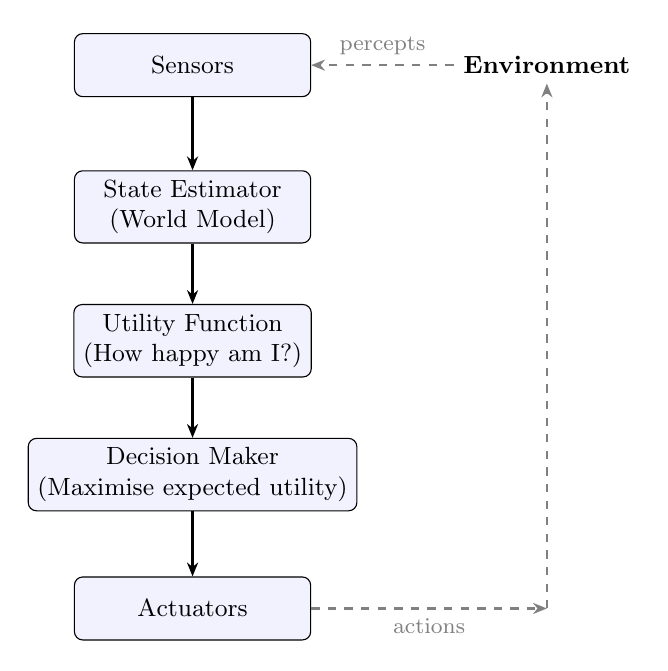
\begin{tikzpicture}[
  box/.style={draw, rounded corners=3pt, minimum width=3cm, minimum height=0.8cm, align=center, fill=blue!5, font=\small},
  arrow/.style={-{Stealth[length=5pt, width=4pt]}, thick}
]
\node[box] (sensors) at (0, 4) {Sensors};
\node[box] (state) at (0, 2.2) {State Estimator\\(World Model)};
\node[box] (utility) at (0, 0.5) {Utility Function\\(How happy am I?)};
\node[box] (decision) at (0, -1.2) {Decision Maker\\(Maximise expected utility)};
\node[box] (actuators) at (0, -2.9) {Actuators};

\node[draw=none, font=\small\bfseries] (env) at (4.5, 4) {Environment};
\node[draw=none, font=\small\bfseries] (env2) at (4.5, -2.9) {};

\draw[arrow] (sensors) -- (state);
\draw[arrow] (state) -- (utility);
\draw[arrow] (utility) -- (decision);
\draw[arrow] (decision) -- (actuators);

% Environment feedback loop
\draw[arrow, dashed, gray] (env) -- (sensors) node[midway, above, font=\footnotesize] {percepts};
\draw[arrow, dashed, gray] (actuators) -- (4.5, -2.9) node[midway, below, font=\footnotesize] {actions};
\draw[arrow, dashed, gray] (4.5, -2.9) -- (env);
\end{tikzpicture}
\end{center}

\subsubsection*{How It Extends Goal-Based Agents}

\begin{center}
\renewcommand{\arraystretch}{1.3}
\begin{tabular}{l|p{6cm}|p{6cm}}
\toprule
\textbf{Aspect} & \textbf{Goal-Based Agent} & \textbf{Utility-Based Agent} \\
\midrule
State evaluation & Binary: goal or not-goal & Continuous: $U(s) \in \mathbb{R}$ — degree of satisfaction \\
Multiple goals & Cannot weigh conflicting goals & Utility function provides unified comparison \\
Uncertainty & No framework — assumes deterministic actions & Expected utility handles probabilistic outcomes \\
Trade-off decisions & Cannot make them & Natural — choose highest utility \\
\bottomrule
\end{tabular}
\end{center}

\begin{notesbox}
\textbf{Real-world example — Autonomous Taxi:} A goal-based taxi's goal is ``arrive at destination.'' A utility-based taxi balances: arrival time, passenger comfort (smooth driving), fuel economy, safety (accident probability), and legal compliance (speed limits) — all combined into a single utility function. When a short, fast route has high accident risk, the utility function correctly prefers a slightly longer, safer route.
\end{notesbox}

\newpage

%=====================================================================
\section{Examination 2021 — Q1 (9.75 Marks)}
%=====================================================================

\begin{solutionbox}
\textbf{Question breakdown:}
\begin{enumerate}[noitemsep]
  \item[(a)] Do Sophia and Jarvis possess features and signs of intelligence? Elaborate considering their behaviour. (1.5)
  \item[(b)] Suppose you design a machine to pass the Turing test. What capabilities must it have? (1)
  \item[(c)] How do Simple Reflex agents differ from Goal-Driven agents considering architecture? (1)
  \item[(d)] Consider ``Amazon Echo'' — PAGE description + environment characterisation. (4)
  \item[(e)] What agent architecture is best for automated taxi driving? Justify. (1.25)
\end{enumerate}
\end{solutionbox}

%----------------------------------------------------------------------
\subsection{Part (a) — Sophia and Jarvis: Signs of Intelligence? \ [1.5 marks]}
%----------------------------------------------------------------------

\subsubsection*{Sophia (Hanson Robotics, 2016)}

\noindent\textbf{Features suggesting intelligence:}
\begin{keypoints}
  \item Human-like facial expressions (30+ motors simulating human facial muscles).
  \item Speech recognition and natural language generation.
  \item Can answer pre-scripted and some open-domain questions.
  \item Physical embodiment with gaze tracking and gesture.
\end{keypoints}

\noindent\textbf{Limitations — why Sophia is NOT truly intelligent:}
\begin{keypoints}
  \item \textbf{Scripted behaviour:} Most interactions are pre-programmed or human-controlled (Wizard-of-Oz). Sophia does not generate original thoughts.
  \item \textbf{No learning:} Sophia's responses do not meaningfully improve through experience.
  \item \textbf{No genuine understanding:} Operates via pattern matching and rule-based responses — no comprehension of what it says.
  \item \textbf{No autonomy:} Cannot set its own goals or adapt to truly novel situations without human scripting.
\end{keypoints}

\noindent\textbf{Verdict:} Sophia exhibits \textbf{simulated} intelligence (acting humanly), not genuine intelligence. It is a sophisticated animatronic puppet with NLP capabilities — a demonstration of engineering, not cognition.

\vspace{0.4em}

\subsubsection*{J.A.R.V.I.S. (Marvel Cinematic Universe — fictional AI)}

\noindent\textbf{Features suggesting intelligence (in fiction):}
\begin{keypoints}
  \item Natural language understanding at expert-human level.
  \item Multi-domain reasoning (engineering, tactics, science, personal assistance).
  \item Controls complex systems (Iron Man suit, building infrastructure) autonomously.
  \item Exhibits personality, humour, and apparent emotional intelligence.
  \item Learns and adapts to Tony Stark's preferences over time.
\end{keypoints}

\noindent\textbf{Reality check:}
\begin{keypoints}
  \item J.A.R.V.I.S. is \textbf{fictional} — no real AI system approaches this level of general intelligence.
  \item The closest real systems are specialised narrow-AI assistants (Siri, Alexa, Google Assistant) which operate on vastly simpler principles.
  \item J.A.R.V.I.S. represents \textbf{Artificial General Intelligence (AGI)} — a goal not yet achieved by any real system.
\end{keypoints}

\begin{answerbox}
\textbf{Conclusion:} Sophia demonstrates \textbf{simulated intelligence} (appearance of intelligence through engineering) while J.A.R.V.I.S. represents \textbf{fictional AGI} (human-level intelligence across all domains). Neither possesses genuine intelligence in the sense of autonomous reasoning, learning, and understanding. Sophia is a scripted NLP system with a robotic face; J.A.R.V.I.S. is a narrative device.
\end{answerbox}

%----------------------------------------------------------------------
\subsection{Part (b) — Capabilities for Passing the Turing Test \ [1 mark]}
%----------------------------------------------------------------------

\noindent A machine designed to pass the Turing Test must possess:

\begin{keypoints}
  \item \textbf{Natural Language Processing:} Understand and generate fluent, contextually appropriate human language in real time.
  \item \textbf{Knowledge Representation:} Store a vast repository of facts, concepts, and relationships — and retrieve them instantly and relevantly.
  \item \textbf{Automated Reasoning:} Draw logical inferences, answer novel questions, and construct coherent arguments from stored knowledge.
  \item \textbf{Machine Learning:} Adapt to the interrogator's style, learn from the conversation, and handle topics not explicitly pre-programmed.
  \item \textbf{Theory of Mind (implicit):} Model what the interrogator knows, believes, and expects — to avoid responses that are obviously non-human.
\end{keypoints}

\noindent For the \textbf{Total Turing Test} (which adds physical interaction), the machine would additionally need:
\begin{keypoints}
  \item \textbf{Computer Vision:} Perceive and recognise objects, people, and gestures.
  \item \textbf{Robotics:} Manipulate objects and navigate physical space.
\end{keypoints}

%----------------------------------------------------------------------
\subsection{Part (c) — Simple Reflex vs Goal-Driven Agents \ [1 mark]}
%----------------------------------------------------------------------

\begin{center}
\renewcommand{\arraystretch}{1.5}
\begin{tabular}{p{4.5cm}|p{5.5cm}|p{5.5cm}}
\toprule
\textbf{Aspect} & \textbf{Simple Reflex Agent} & \textbf{Goal-Driven Agent} \\
\midrule
\textbf{Decision basis} &
  Current percept only &
  Current percept + explicit goal + predicted future states \\
\midrule
\textbf{Internal state} &
  None (stateless) &
  World model + goal state \\
\midrule
\textbf{Action selection} &
  Condition–action rules: \textbf{IF} \textit{percept} \textbf{THEN} \textit{action} &
  Search/planning: find action sequence that transforms current state to goal state \\
\midrule
\textbf{Looks ahead?} &
  No — reacts to the present &
  Yes — considers future consequences of actions \\
\midrule
\textbf{Architecture} &
  Sensor $\to$ Rule matcher $\to$ Actuator &
  Sensor $\to$ State estimator $\to$ Goal comparator $\to$ Planner $\to$ Actuator \\
\midrule
\textbf{When appropriate} &
  Fully observable, simple stimulus–response mappings (thermostat, spam filter) &
  Requires planning, sequential decisions (navigation, puzzle solving, route finding) \\
\midrule
\textbf{Limitation} &
  Cannot handle partial observability; no long-term planning &
  Computationally more expensive; requires search/planning algorithms \\
\bottomrule
\end{tabular}
\end{center}

\begin{answerbox}
\textbf{Key difference:} Simple Reflex = \textbf{react}; Goal-Driven = \textbf{plan}. The reflex agent asks ``What should I do right now based on what I see?'' The goal-driven agent asks ``What sequence of actions will get me from here to my goal?''
\end{answerbox}

%----------------------------------------------------------------------
\subsection{Part (d) — Amazon Echo: PAGE + Environment \ [4 marks]}
%----------------------------------------------------------------------

\subsubsection*{(i) PAGE Description}

\begin{center}
\renewcommand{\arraystretch}{1.5}
\begin{tabular}{l|p{13cm}}
\toprule
\textbf{P} — Percepts &
\textbf{Audio:} Voice commands via far-field microphone array (7 microphones).\\
& \textbf{Touch:} Physical button presses (volume, mute, action button).\\
& \textbf{Network:} WiFi connectivity status, API responses, streaming data.\\
\midrule
\textbf{A} — Actions &
\textbf{Audio output:} Speech synthesis (Alexa voice), music playback, notification sounds.\\
& \textbf{Visual:} LED ring indicating status (listening, processing, muted, notification).\\
& \textbf{Network:} API calls to cloud services (weather, news, calendar, shopping), smart home device control (lights, thermostats, locks).\\
& \textbf{Display (Echo Show):} Show visual information, video calls.\\
\midrule
\textbf{G} — Goals &
Respond accurately to user voice commands.\\
& Provide timely information (weather, news, reminders, calendar).\\
& Control smart home devices reliably.\\
& Maintain user privacy and data security.\\
& Minimise false activations (wake word detection).\\
\midrule
\textbf{E} — Environment &
\textbf{Physical:} Home/office indoor environment — rooms with varying acoustics, background noise, multiple speakers.\\
& \textbf{Digital:} Cloud services, smart home ecosystem, internet.\\
& \textbf{Social:} Multiple users with different voices, accents, languages, and authorisation levels.\\
\bottomrule
\end{tabular}
\end{center}

\subsubsection*{(ii) Environment Characterisation}

\begin{center}
\renewcommand{\arraystretch}{1.4}
\begin{tabular}{l|l|p{8cm}}
\toprule
\textbf{Dimension} & \textbf{Classification} & \textbf{Justification} \\
\midrule
\textbf{Accessibility} (Observability) & \textbf{Inaccessible} (Partially observable) & Echo cannot see users' faces, gestures, or context. It only hears audio within microphone range. User intent is inherently hidden — the same utterance (``play Despacito'') could mean different things. \\
\midrule
\textbf{Determinism} & \textbf{Non-deterministic} (Stochastic) & The same command may produce different results depending on network state, cloud service availability, background noise, and user's subscription status. Voice recognition itself is probabilistic. \\
\midrule
\textbf{Episodicity} & \textbf{Episodic} (mostly) & Most interactions are independent: asking the weather does not affect the next music request. However, multi-turn dialogues (``Alexa, what's the weather? — And tomorrow?'') make it partially sequential. \\
\midrule
\textbf{Dynamism} & \textbf{Dynamic} & The environment changes while Echo is processing (new sounds, new people speaking). However, Echo can ask for clarification (``Sorry, I didn't catch that''), making it adaptable to dynamism. \\
\midrule
\textbf{Continuity} & \textbf{Discrete} & Commands are discrete utterances; actions are discrete API calls; responses are discrete audio segments. Volume is continuous but the agent's decision space is discrete. \\
\midrule
\textbf{Agency} & \textbf{Multi-agent} & Multiple users interact with Echo; Echo interacts with cloud services (other software agents); in multi-Echo households, devices coordinate. \\
\bottomrule
\end{tabular}
\end{center}

%----------------------------------------------------------------------
\subsection{Part (e) — Best Architecture for Automated Taxi \ [1.25 marks]}
%----------------------------------------------------------------------

\begin{answerbox}
\textbf{Recommended: Utility-Based Agent}

\noindent\textbf{Justification:}
\begin{keypoints}
  \item An automated taxi faces \textbf{conflicting objectives} that must be balanced — passenger safety, trip time, fuel efficiency, passenger comfort, legal compliance, and fare optimisation.
  \item The environment is \textbf{stochastic} — other drivers, pedestrians, weather, and traffic conditions are unpredictable. A utility-based agent can make optimal decisions under uncertainty using \textbf{expected utility maximisation}.
  \item A \textbf{pure goal-based agent} (``arrive at destination'') would take unacceptable risks — maximising speed and running red lights if those were the fastest path to the goal.
  \item A \textbf{utility function} encodes the trade-offs: $U = w_1 \cdot \text{safety} + w_2 \cdot (-\text{time}) + w_3 \cdot (-\text{cost}) + w_4 \cdot \text{comfort} + \ldots$, where weights $w_i$ reflect the importance of each objective.
  \item The taxi must also incorporate \textbf{learning} — improving its driving policy from millions of miles of experience, adapting to local driving norms — but the core decision-making architecture is utility-based.
\end{keypoints}

\noindent In practice, modern self-driving systems (Waymo, Cruise) use a \textbf{hybrid} approach: utility-based planning for route-level decisions, with reflex layers for immediate safety (emergency braking), and deep learning for perception and behaviour prediction.
\end{answerbox}

\newpage

%=====================================================================
\section{Examination 2020 — Q1 (9 Marks)}
%=====================================================================

\begin{solutionbox}
\textbf{Question breakdown:}
\begin{enumerate}[noitemsep]
  \item[(a)] What is AI? Explain four approaches: Thinking Humanly, Thinking Rationally, Acting Humanly, Acting Rationally — with examples. (2)
  \item[(b)] What is an intelligent agent? Describe the structure of a learning agent with diagram — four components and their interactions. (3)
  \item[(c)] Mars Rover scenario — percepts, environment, actions, performance, architecture. (4)
\end{enumerate}
\end{solutionbox}

%----------------------------------------------------------------------
\subsection{Part (a) — Four Approaches to AI \ [2 marks]}
%----------------------------------------------------------------------

\noindent AI can be understood through \textbf{four distinct but complementary approaches}, organised along two axes: \textit{reasoning vs.\ behaviour} and \textit{human-like vs.\ rational}.

\vspace{0.5em}

\noindent\textbf{1. Thinking Humanly — Cognitive Modelling Approach}

\begin{keypoints}
  \item \textbf{Goal:} Build computer programs that think the way humans think.
  \item \textbf{Method:} Study human cognition through psychological experiments, then implement computational models that replicate the observed cognitive processes.
  \item \textbf{Requires:} A scientific theory of the mind — how does the human brain represent knowledge, reason, and learn?
  \item \textbf{Example:} The \textbf{General Problem Solver (GPS)} by Newell \& Simon (1961) — modelled human problem-solving by tracking the difference between current and desired states. \textbf{ACT-R} and \textbf{SOAR} are modern cognitive architectures that simulate human memory, learning, and decision-making.
  \item \textbf{Validation:} Compare the model's behaviour (response times, error patterns, eye movements) with human subjects.
\end{keypoints}

\vspace{0.4em}

\noindent\textbf{2. Thinking Rationally — Laws of Thought Approach}

\begin{keypoints}
  \item \textbf{Goal:} Build systems that reason according to irrefutable logical principles.
  \item \textbf{Method:} Formalise problems in mathematical logic; use inference rules (modus ponens, resolution) to derive conclusions from premises.
  \item \textbf{Foundation:} Aristotle's syllogisms — patterns of argument that always yield correct conclusions from correct premises.
  \item \textbf{Example:} \textbf{Theorem provers} (e.g., Prolog, Coq) — given axioms of arithmetic, prove that ``there are infinitely many prime numbers.'' Expert systems like \textbf{MYCIN} used logical rules to diagnose bacterial infections.
  \item \textbf{Limitation:} Pure logic struggles with uncertainty, incomplete knowledge, and problems where the ``correct'' answer depends on context — most real-world problems are not purely logical.
\end{keypoints}

\vspace{0.4em}

\noindent\textbf{3. Acting Humanly — Turing Test Approach}

\begin{keypoints}
  \item \textbf{Goal:} Create systems whose behaviour is indistinguishable from human behaviour.
  \item \textbf{Method:} The Turing Test (1950) — an operational definition: if a human interrogator cannot tell the machine from a human through conversation, the machine exhibits intelligence.
  \item \textbf{Required capabilities:} NLP, knowledge representation, automated reasoning, machine learning.
  \item \textbf{Example:} \textbf{ChatGPT, Claude, Gemini} — LLMs that engage in convincingly human-like conversation across diverse topics. \textbf{ELIZA} (1966) was an early example that simulated a Rogerian psychotherapist using simple pattern matching.
  \item \textbf{Critique:} Passing the Turing Test may require \emph{deception} rather than \emph{intelligence} — a system could pass by being evasive, humorous, or simulating human flaws. The test measures behavioural indistinguishability, not genuine understanding.
\end{keypoints}

\vspace{0.4em}

\noindent\textbf{4. Acting Rationally — Rational Agent Approach}

\begin{keypoints}
  \item \textbf{Goal:} Build agents that act to achieve the best possible outcome (or best expected outcome under uncertainty).
  \item \textbf{Method:} Define a performance measure; for every possible percept sequence, select the action that maximises expected performance.
  \item \textbf{Foundation:} Decision theory, utility theory, probability theory.
  \item \textbf{Example:} \textbf{Self-driving cars} — perceive the road environment (cameras, LIDAR, GPS), plan a safe and efficient route, execute driving actions. \textbf{Chess engines} (Stockfish, AlphaZero) — evaluate positions and select moves that maximise winning probability.
  \item \textbf{Advantage over Acting Humanly:} Rationality is \textbf{mathematically defined} and \textbf{universal} — it does not depend on mimicking human quirks. A calculator acts rationally (correct arithmetic) but not humanly (a human might make errors).
\end{keypoints}

\begin{answerbox}
\textbf{The rational agent approach is the modern standard} in AI textbooks (Russell \& Norvig) because:
\begin{enumerate}[noitemsep]
  \item It is more \textbf{general} than ``thinking humanly'' — not limited by human cognitive biases.
  \item It is more \textbf{tractable} than ``thinking rationally'' — can handle uncertainty where pure logic fails.
  \item It is more \textbf{principled} than ``acting humanly'' — mathematical optimality rather than behavioural mimicry.
\end{enumerate}
\end{answerbox}

%----------------------------------------------------------------------
\subsection{Part (b) — Learning Agent Structure \ [3 marks]}
%----------------------------------------------------------------------

\subsubsection*{What is an Intelligent Agent?}

\noindent An \textbf{intelligent agent} is an entity that perceives its environment through \textbf{sensors} and acts upon it through \textbf{actuators} to maximise its performance measure. The agent function $f: P^* \to A$ maps every possible percept history to an action.

\subsubsection*{The Learning Agent Architecture}

\noindent A learning agent has \textbf{four conceptual components} that work together to enable improvement over time:

\begin{center}
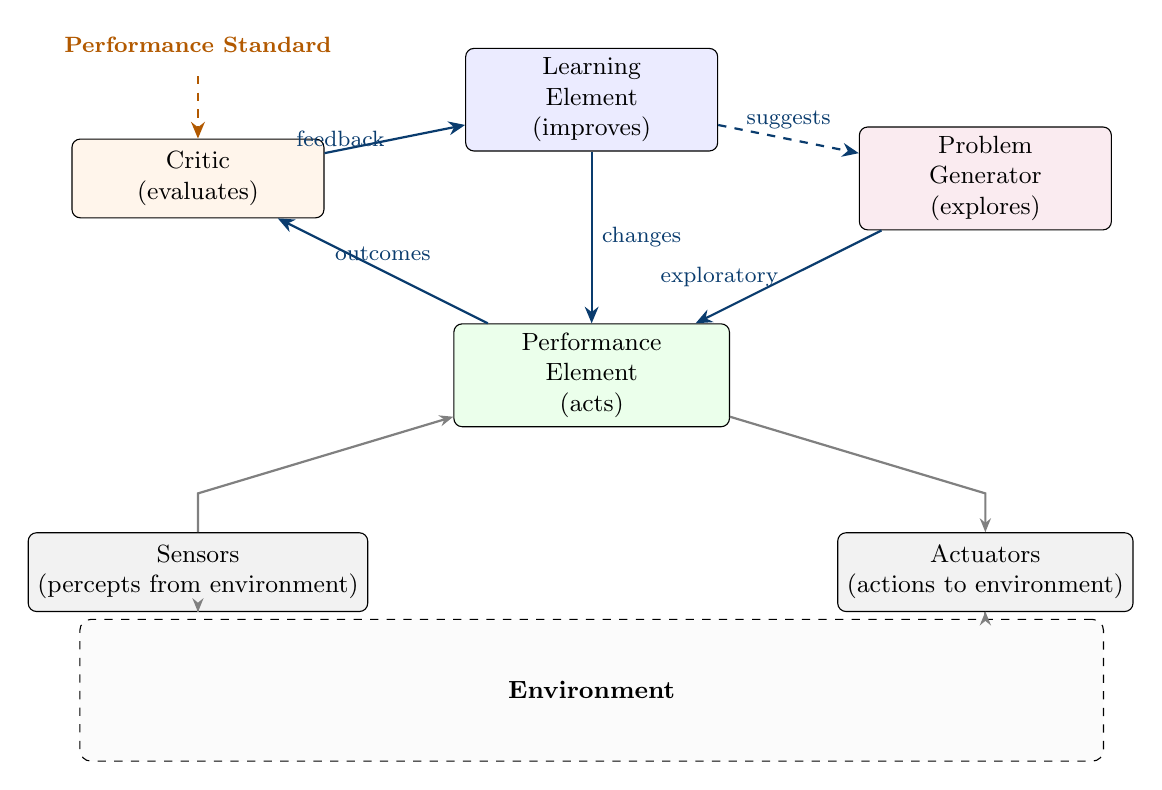
\begin{tikzpicture}[
  box/.style={draw, rounded corners=3pt, minimum width=3.2cm, minimum height=1cm, align=center, fill=blue!5, font=\small},
  arrow/.style={-{Stealth[length=6pt, width=5pt]}, thick, color=sectionblue},
  grayarrow/.style={-{Stealth[length=5pt, width=4pt]}, thick, gray}
]

% Performance element (center)
\node[box, fill=green!8, minimum width=3.5cm, minimum height=1.3cm] (pe) at (0, 0)
  {Performance\\Element\\(acts)};

% Critic (left)
\node[box, fill=orange!8] (critic) at (-5, 2.5) {Critic\\(evaluates)};

% Learning element (top)
\node[box, fill=blue!8] (learner) at (0, 3.5) {Learning\\Element\\(improves)};

% Problem generator (right)
\node[box, fill=purple!8] (pg) at (5, 2.5) {Problem\\Generator\\(explores)};

% Sensors and actuators
\node[box, fill=gray!10] (sensors) at (-5, -2.5) {Sensors\\(percepts from environment)};
\node[box, fill=gray!10] (actuators) at (5, -2.5) {Actuators\\(actions to environment)};

% Environment
\node[draw, dashed, rounded corners, minimum width=13cm, minimum height=1.8cm, fill=gray!3] (env) at (0, -4) {};
\node[font=\small\bfseries, draw=none] at (0, -4) {Environment};

% Arrows
\draw[grayarrow] (sensors) -- (-5, -1.5) -- (pe);
\draw[grayarrow] (pe) -- (5, -1.5) -- (actuators);
\draw[arrow] (critic) -- node[midway, left, font=\footnotesize] {feedback} (learner);
\draw[arrow] (learner) -- node[midway, right, font=\footnotesize] {changes} (pe);
\draw[arrow] (pg) -- node[midway, left, font=\footnotesize] {exploratory} (pe);
\draw[arrow] (pe) -- node[midway, above, font=\footnotesize] {outcomes} (critic);
\draw[arrow, dashed] (learner) -- node[midway, above, font=\footnotesize] {suggests} (pg);

% Percept arrow from env
\draw[grayarrow, dashed] (-5, -3) -- (sensors);
\draw[grayarrow, dashed] (actuators) -- (5, -3);

% Performance standard
\node[draw=none, font=\footnotesize\bfseries, color=orange!70!black] at (-5, 4.2) {Performance Standard};
\draw[arrow, dashed, orange!70!black] (-5, 3.8) -- (critic);

\end{tikzpicture}
\end{center}

\vspace{0.5em}

\noindent\textbf{Component 1 — Performance Element (``The Actor'')}
\begin{keypoints}
  \item This is the agent's \textbf{action-selection mechanism} — it takes in percepts and outputs actions. It is the same as the entire agent in a non-learning architecture.
  \item Initially, it may be simple (e.g., random actions or basic rules). The learning element \textbf{modifies} it over time to improve performance.
  \item \emph{Example:} In a chess agent, the performance element is the move-selection function (evaluation + minimax). It gets better as the learning element updates the evaluation weights.
\end{keypoints}

\noindent\textbf{Component 2 — Critic (``The Evaluator'')}
\begin{keypoints}
  \item Compares the agent's actual behaviour against a \textbf{fixed, externally-defined performance standard}.
  \item Tells the learning element: ``You did well here'' or ``You did poorly here.''
  \item \textbf{Critical distinction:} The critic uses a \textbf{fixed} standard — it does not change. This prevents the agent from ``moving the goalposts'' to declare itself successful.
  \item \emph{Example:} In chess, the critic observes whether the agent won or lost — an objective, external outcome. It does not judge the agent's intentions or effort.
\end{keypoints}

\noindent\textbf{Component 3 — Learning Element (``The Improver'')}
\begin{keypoints}
  \item Takes feedback from the critic and \textbf{modifies the performance element} to do better in future.
  \item This is where the actual \textbf{learning algorithm} lives — neural network weight updates, rule refinement, value function updates, etc.
  \item \emph{Example:} In chess, the learning element adjusts evaluation weights — if losing positions were previously evaluated as equal, the weights are corrected so similar positions are recognised as bad in future.
\end{keypoints}

\noindent\textbf{Component 4 — Problem Generator (``The Explorer'')}
\begin{keypoints}
  \item Suggests \textbf{exploratory actions} that may not be optimal in the short term but lead to \textbf{new, informative experiences} that improve long-term performance.
  \item Addresses the \textbf{exploration vs.\ exploitation} dilemma — without exploration, the agent would repeat what it already knows and never discover better strategies.
  \item \emph{Example:} In chess, the problem generator might suggest trying a novel opening (suboptimal short-term) to learn whether it leads to winning positions — knowledge that improves future games.
\end{keypoints}

\subsubsection*{How the Four Components Interact}

\begin{enumerate}[noitemsep, leftmargin=1.5cm]
  \item The \textbf{performance element} selects actions based on current knowledge.
  \item The \textbf{critic} observes outcomes and provides feedback against a fixed standard.
  \item The \textbf{learning element} uses this feedback to modify the performance element.
  \item The \textbf{problem generator} occasionally overrides the performance element to explore new behaviours.
  \item The outcomes of these exploratory actions are then evaluated by the critic, feeding back into the learning element — closing the loop.
\end{enumerate}

\begin{answerbox}
\textbf{The learning agent is the most general architecture.} It subsumes all simpler architectures: a Simple Reflex, Model-Based, Goal-Based, or Utility-Based agent can each be the ``performance element'' that the learning element improves over time.
\end{answerbox}

%----------------------------------------------------------------------
\subsection{Part (c) — Mars Rover \ [4 marks]}
%----------------------------------------------------------------------

\noindent\textbf{Note:} The Mars Rover scenario also appears in the 2023 Q1. The model answer below is tailored to the 2020 exam context — which may have asked about a single generic Mars Rover rather than two specific rovers. The core analysis is transferable.

\subsubsection*{(i) Percepts (Sensory Inputs)}

\begin{keypoints}
  \item \textbf{Visual:} Panoramic cameras (Pancam/MastCam), navigation cameras (Navcam), hazard avoidance cameras (Hazcam), microscopic imager.
  \item \textbf{Spectroscopic:} X-ray spectrometer, laser-induced breakdown spectroscopy (LIBS), alpha particle X-ray spectrometer — for chemical and mineral composition.
  \item \textbf{Environmental:} Temperature, atmospheric pressure, wind speed/direction, humidity, ultraviolet radiation sensors.
  \item \textbf{Navigational:} Wheel odometry, inertial measurement unit (IMU), sun sensor for orientation.
  \item \textbf{Communication:} Signal strength from Earth and Mars orbiters.
  \item \textbf{Internal:} Power levels (battery + RTG), actuator temperatures, instrument health telemetry.
\end{keypoints}

\subsubsection*{(ii) Environment Characterisation}

\begin{center}
\renewcommand{\arraystretch}{1.3}
\begin{tabular}{l|l|p{8.5cm}}
\toprule
\textbf{Dimension} & \textbf{Class} & \textbf{Reasoning} \\
\midrule
Observability & Partially observable & Hidden subsurface structures, occluded terrain, unexpected soil properties. \\
Determinism & Stochastic & Unpredictable terrain slippage, dust storm interference, communication latency. \\
Episodicity & Sequential & Every action (traverse, drill) permanently changes the rover's state and position. \\
Dynamism & Semi-dynamic & Environment changes slowly (seasons, dust accumulation) but not during deliberation. \\
Continuity & Continuous & Position, speed, temperature, radiation — all continuous variables. \\
Agency & Single-agent & One rover operates independently at its landing site; communication with Earth is remote operation, not agent interaction. \\
\bottomrule
\end{tabular}
\end{center}

\subsubsection*{(iii) Actions}

\begin{keypoints}
  \item \textbf{Autonomous navigation:} Drive to target coordinates while avoiding hazards using stereo vision and terrain analysis.
  \item \textbf{Scientific observation:} Point instruments at targets, capture images and spectra, analyse data onboard.
  \item \textbf{Sample analysis:} Drill/abrade rocks, collect powder, deliver to internal laboratory instruments.
  \item \textbf{Communication:} Uplink science data and telemetry to orbiters for relay to Earth; receive commands from Earth.
  \item \textbf{Power/thermal management:} Activate heaters, enter low-power safe mode during unfavourable conditions.
  \item \textbf{Fault recovery:} Detect anomalies (stuck wheels, instrument failure), diagnose, attempt recovery or await Earth instructions.
\end{keypoints}

\subsubsection*{(iv) Performance Evaluation}

\begin{keypoints}
  \item \textbf{Science output:} Number of rock/soil samples analysed; significant discoveries (evidence of past water, organic molecules, habitable environments).
  \item \textbf{Mission longevity:} Total operational days vs.\ planned primary mission duration.
  \item \textbf{Distance covered:} Total kilometres driven across the Martian surface.
  \item \textbf{Autonomy rate:} Percentage of driving decisions made autonomously without Earth-in-the-loop.
  \item \textbf{Data returned:} Total volume of science and engineering data transmitted to Earth.
  \item \textbf{Survival:} Number and severity of fault events successfully handled.
\end{keypoints}

\subsubsection*{(v) Most Appropriate Agent Architecture}

\begin{answerbox}
\textbf{Recommended: Model-Based + Goal-Based Hybrid Agent}

\noindent\textbf{Justification:}
\begin{keypoints}
  \item \textbf{Model-Based (necessary):} The rover must track its position, terrain map, instrument states, and resource levels because direct observation is incomplete. It maintains an internal world model updated by percepts.
  \item \textbf{Goal-Based (necessary):} Daily operations involve explicit goals — ``drive to waypoint X, examine rock Y with instrument Z.'' The rover must plan action sequences to achieve these goals. Simple reflex rules are insufficient for autonomous kilometre-scale navigation through unknown terrain.
  \item \textbf{Why not purely Utility-Based?} For the 2020-era rover, objectives are relatively well-defined and hierarchically structured (survival > communication > science), limiting the need for complex utility trade-offs. A goal-based approach with priority ordering is sufficient and computationally simpler.
  \item \textbf{Why Learning is secondary (for 2020):} While modern rovers incorporate ML for terrain classification, the core decision loop (plan $\to$ execute $\to$ monitor $\to$ replan) is goal-driven. The learning augments but does not replace the goal-based architecture.
\end{keypoints}
\end{answerbox}

\newpage

%=====================================================================
\section{Quick Reference — Exam Execution}
%=====================================================================

\subsection*{The 3-Part Q1 Template (Every Year)}

\noindent Every Q1 paper from 2020–2024 follows the same structure. When answering, use this mental template:

\begin{center}
\renewcommand{\arraystretch}{1.4}
\begin{tabular}{c|p{5.5cm}|p{5.5cm}|p{5.5cm}}
\toprule
\textbf{Part} & \textbf{What it asks} & \textbf{Your answer framework} & \textbf{Typical marks} \\
\midrule
\textbf{Part 1} & Define AI / AI approaches / AI vs ML & 4 approaches (2$\times$2 matrix) or AI $\supset$ ML $\supset$ DL hierarchy & 1--2 \\
\midrule
\textbf{Part 2} & Turing Test — evaluate [system X] & (i) How it corresponds (5 points) + (ii) Limitations (5 points) & 2.5--3 \\
\midrule
\textbf{Part 3} & [Scenario] — percepts, environment, actions, performance, architecture & PAGE + 6 environment dimensions + architecture recommendation with justification & 4 \\
\bottomrule
\end{tabular}
\end{center}

\subsection*{Architecture Selection Quick Guide}

\begin{center}
\renewcommand{\arraystretch}{1.4}
\begin{tabular}{l|l|l}
\toprule
\textbf{If the scenario involves\ldots} & \textbf{Recommend} & \textbf{Key justification phrase} \\
\midrule
Only current sensor reading matters; simple rules suffice & Simple Reflex & ``Direct condition-action mapping'' \\
Cannot see everything; must remember & Model-Based & ``Maintains internal state to handle partial observability'' \\
Must plan a sequence of actions toward an objective & Goal-Based & ``Searches/plans to find action sequences achieving explicit goals'' \\
Multiple conflicting objectives; uncertainty & Utility-Based & ``Utility function provides unified comparison of trade-offs'' \\
Environment is unknown or changing; must improve & Learning Agent & ``Improves performance from experience via critic + learning element'' \\
\midrule
\end{tabular}
\end{center}

\subsection*{Environment Characterisation Quick Guide}

\begin{center}
\renewcommand{\arraystretch}{1.4}
\begin{tabular}{l|l}
\toprule
\textbf{Scenario} & \textbf{Likely classification} \\
\midrule
Mars Rover & Partially observable, Stochastic, Sequential, Semi-dynamic, Continuous, Single-agent \\
Self-driving Taxi & Partially observable, Stochastic, Sequential, Dynamic, Continuous, Multi-agent \\
Robot Vacuum & Partially observable, Stochastic, Sequential, Dynamic, Continuous, Single-agent \\
Agricultural Robot & Partially observable, Stochastic, Sequential, Dynamic, Continuous, Single-agent \\
Amazon Echo / Alexa & Partially observable, Stochastic, Episodic (mostly), Dynamic, Discrete, Multi-agent \\
Chess AI & Fully observable, Deterministic, Sequential, Static, Discrete, Multi-agent (competitive) \\
\bottomrule
\end{tabular}
\end{center}

\end{document}
